\chapter{Preprocessing}\label{preprocessing}

Le immagini raw nei dataset sono sufficenti ad una \gls{cnn} per ottenere buoni risultati, ma è possibile migliorare i risultati attraverso una preleaborazione delle immagini, in particolare la rimozione di artefatti, rimozione del rumore e migliora la qualità e
produce un'immagine in cui le feacture  possono essere estratte correttamente\cite{permual_contrast}

\section{Contrasto}\label{contrasto}

Il contrasto è la differenza tra la massima e la minima
intensità dei pixel. 

Il contrasto si può aggiustare secondo determinati valori statici, oppure secondo tecniche più raffinate, per esempio attraverso la deviazione standard e la media. 

Un metodo più raffinato è la stima del MSE e PSNR. Nel processo di miglioramento del contrasto, i pixel con
valore di pixel più basso di un valore specifico vengono visualizzati come
nero, mentre i pixel con un valore di pixel più alto vengono
visualizzato come bianco, e i pixel che hanno un valore di pixel
tra questi due valori vengono visualizzati come tinta di grigio.
Il risultato di questo processo è una mappatura lineare di un
sottoinsieme di valori di pixel all'intera gamma di grigi da
nero al bianco, creando un'immagine di maggiore contrasto. 

L'algoritmo di stiramento del contrasto è usato per allungare
la gamma dei valori di colore per usare tutti i valori possibili per
migliorare il contrasto. Per preservare l'accurata proporzione del colore
quando viene usato l'algoritmo di stiramento del contrasto,
viene applicata una scalatura simile per lo stretching di tutti i canali. Nel primo
passo i canali rosso e verde sono bilanciati per essere il canale blu
leggermente il canale blu, allungando l'istogramma su entrambi i lati per ottenere
istogramma ben distribuito.

Qui il peak signal-to-noise ratio (PSNR), cioè un indicatore di qualità dell'immagine è calcolato usando l'equazione:

\[ \operatorname{PSNR}=10 \cdot \log _{10}\left(\frac{\operatorname{MAX}_{1}^{2}}{\operatorname{MSE}}\right) \]

Il PSNR è ben definito semplicemente attraverso l'errore quadratico medio (MSE).
Le immagini monocromatiche \(m\times n\) prive di rumore I e la sua approssimazione rumorosa K è data allora MSE è definito come:

\[ \operatorname{MSE}=\frac{1}{m n} \sum_{i=0}^{m-1} \sum_{j=0}^{n-1}[I(i, j)-K(i, j)]^{2} \]

Una volta determinato il PSNR è possibile effettuare una equalizzazione dell'istogramma per aggiustare il contrasto come mostrato in \cref{fig:histogram}\cite{pandey_contrast}\cite{permual_contrast}\cite{hummel_histogram}.

\begin{figure}[ht]
    \centering
    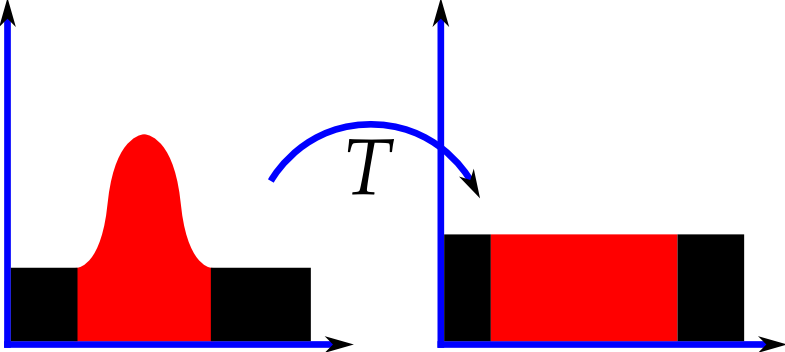
\includegraphics[width=0.7\textwidth]{preprocessing/histogram.png}
    \caption{Metodo dell'equalizzazione dell'istogramma}
    \label{fig:histogram}
\end{figure}

\paragraph{CLAHE}\label{clahe}

Una tecnica più avanzata per migliorare il contrasto nelle immagini è la contrast limited adaptive histogram equalization (CLAHE) che a differenza della classica equalizizazione dell'istogramma divide l'immagini in tante sottoimmagini e per ogni sottoimmagine calcola l'istogramma ed effettua il miglioramento del contrasto, come mostrato in \cref{fig:clahe}\cite{hummel_histogram}.


\begin{figure}[ht]
    \centering
    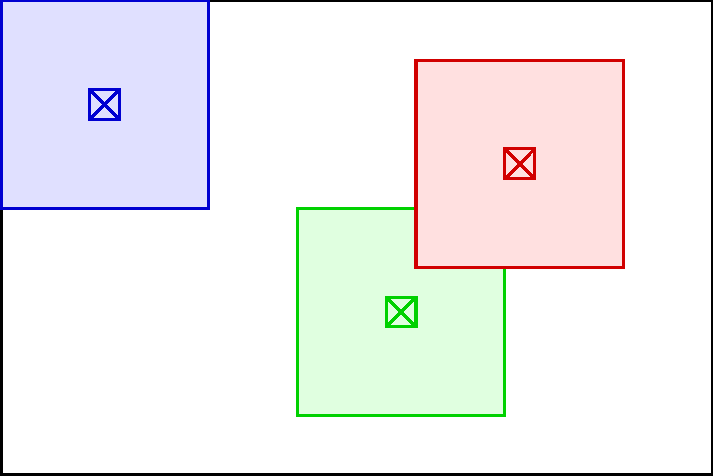
\includegraphics[width=0.7\textwidth]{preprocessing/clahe.pdf}
    \caption{Metodo dell'equalizzazione dell'istogramma}
    \label{fig:clahe}
\end{figure}

\section{Filtro bilaterale}\label{filtro-bilaterale}

Per la rimozione del rimozione del rumore  è stato scelto un  filtro bilaterale è stato scelto per la rimozione del rumore perché conserva
e migliora le caratteristiche che sono utili nelle fasi di addestramento\cite{narbalata_larynge}.